\section{Führe die Katze}
In dieser Aufgabe bauen wir ein kleines Spiel. Es soll eine Katze auf einer Rennbahn geführt werden ohne, dass die Wand berührt werden darf. Einige von euch kennen ein ähnliches Spiel unter dem Namen \emph{heißer Draht}.
\subsection{Male eine Rennbahn}
Wir brauchen eine Rennbahn für unsere Hauptfigur. Wir erzeugen dazu ein weiteres Sprite.
\begin{itemize}
\item[1. ] Klicke auf das \textit{Neues Objekt malen}-Icon
\end{itemize}
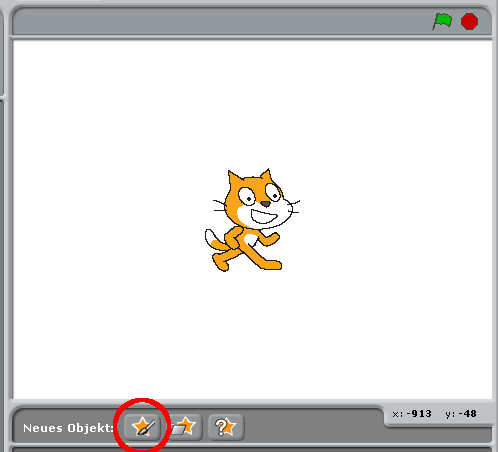
\includegraphics[width=0.6\textwidth]{images/aufgabe4_neues_objekt_malen.png}
\begin{itemize}
\item[2. ] Benutze das Zoom-Tool um komplett herauszuzoomen. Klicke auf die Minus-Lupe.
\end{itemize}
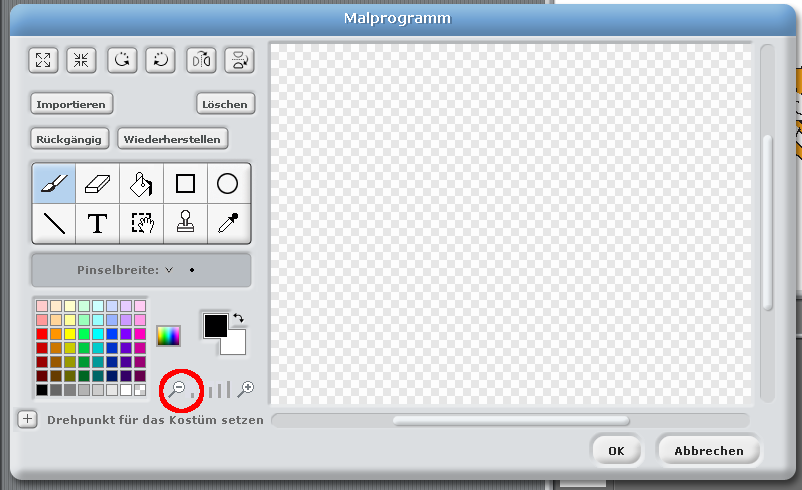
\includegraphics[width=0.6\textwidth]{images/aufgabe4_zoom.png}
\begin{itemize}
\item[3. ] Klicke auf den Pinsel um diesen auszuwählen, wähle einen dickeren Pinsel und die Farbe grau.
\end{itemize}
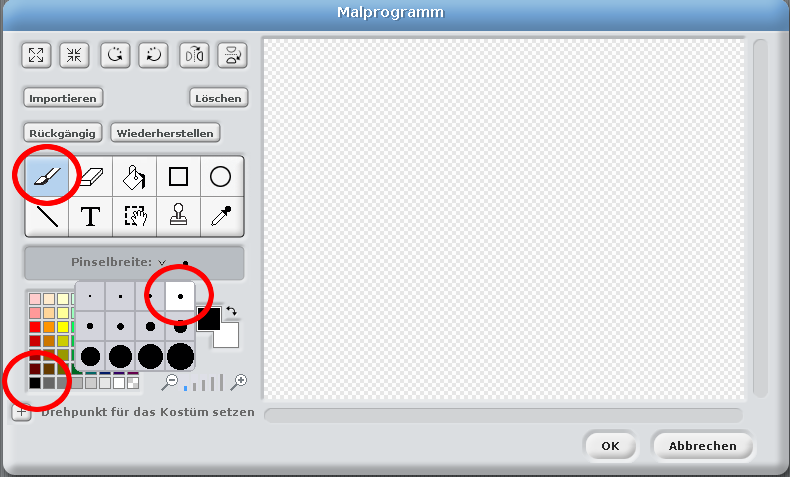
\includegraphics[width=0.6\textwidth]{images/aufgabe4_rennbahn_pinsel_waehlen.png}
\begin{itemize}
\item[4. ] Benutze den Pinsel um eine Rennbahn zu malen.
\end{itemize}
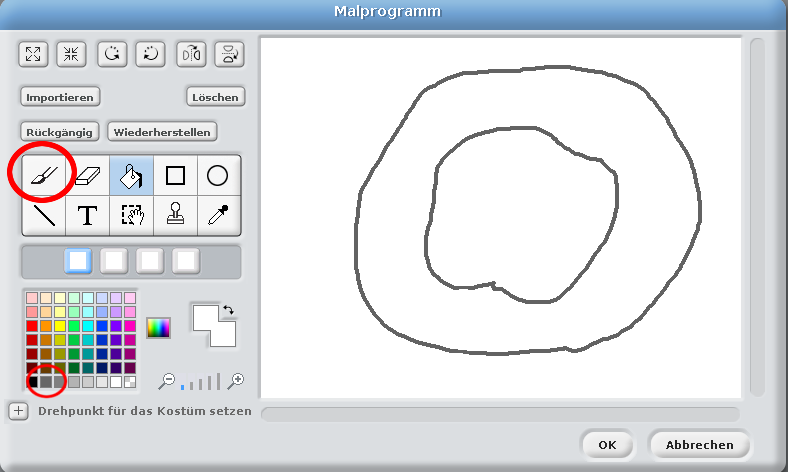
\includegraphics[width=0.6\textwidth]{images/aufgabe4_rennbahn_malen_00.png}
\begin{itemize}
\item[5. ] Da das jetzt einer Rennbahn noch nicht so ähnlich sieht füllen wir die Rennfläche mit der Farbe \emph{hellgrün} und den Berg in der Mitte mit der Farbe \emph{braun} und alles andere Hellblau. Du kannst die Flächen mit dem Pinsel anmalen, leichter ist es jedoch mit dem \emph{Farbeimer}. Dazu einfach den Farbeimer und die Farbe auswählen und dann auf die gewünschte Fläche klicken.
\end{itemize}
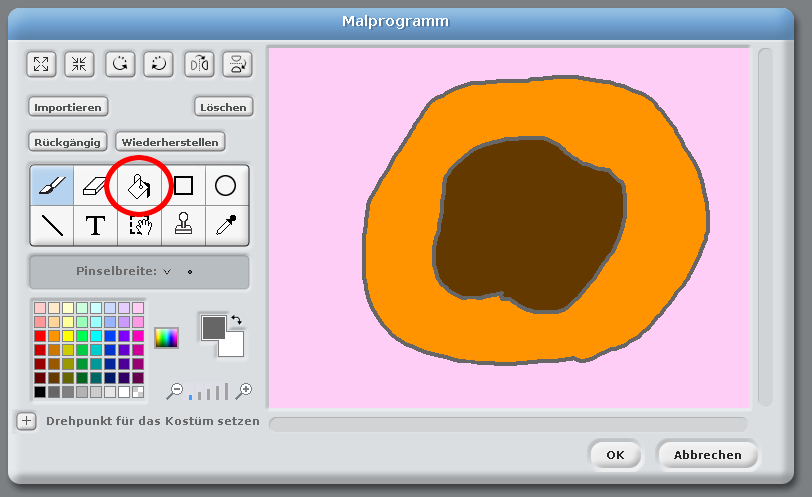
\includegraphics[width=0.6\textwidth]{images/aufgabe4_rennbahn_malen_01.png}
\begin{itemize}
\item[6. ] Zum Schluss fügen wir noch ein weiteren Sprite hinzu und zwar eine \emph{Start/Ziel-Linie} in der Farbe \emph{rot}, diese erstellen und auf die gewünschte Position schieben.
\end{itemize}
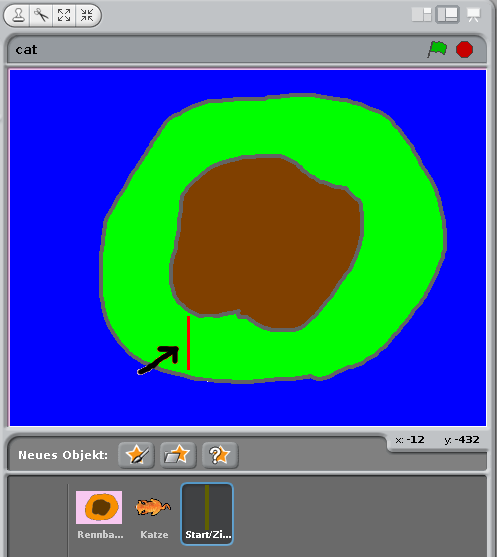
\includegraphics[width=0.6\textwidth]{images/aufgabe4_rennbahn_malen_02.png}
\begin{itemize}
\item[7.] Ändere den Namen des Sprites zu \textit{Rennbahn} und den Namen des Sprites für die Start/Ziel-Linie zu \textit{Start/Ziel}.
\end{itemize}

\subsection{Katze einfügen}

\begin{itemize}
\item[1.] Füge den Sprite \emph{Katze} aus einer Datei hinzu.
\end{itemize}
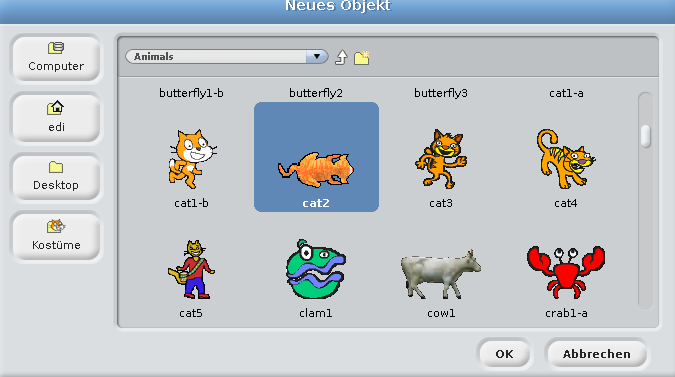
\includegraphics[width=0.6\textwidth]{images/aufgabe4_katze_sprite.png}
\begin{itemize}
\item[2. ] Ändere den Namen des Sprites zu Katze.
\end{itemize}
\begin{itemize}
\item[3.] Benutze das Verkleinerungs-Tool, um die Größe deiner Katze soweit zu verkleinern, dass sie zur Größe der Bahn passt und ohne anzustoßen auf der Bahn laufen kann.
\end{itemize}
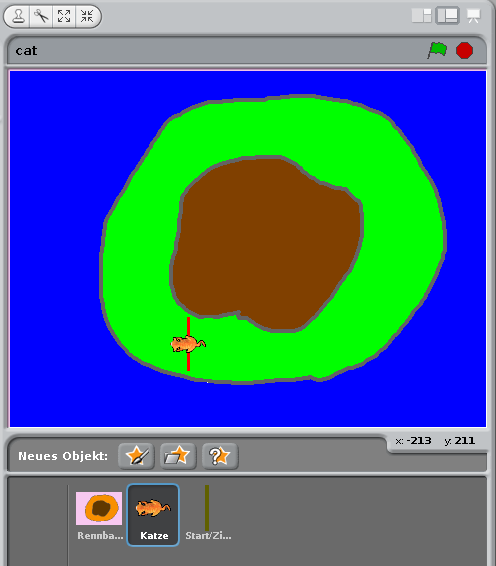
\includegraphics[width=0.6\textwidth]{images/aufgabe4_katze_schrumpfen.png}

\subsection{Erzeuge das Script für die Steuerung der Katze}

\begin{itemize}
\item[1. ] Klicke auf den Sprite Katze.
\item[2. ] Ziehe folgende Kacheln in dein Skript-Panel:
  \begin{itemize}
  \item[1. ] Aus dem Steuerungs-Panel die Kachel \textit{Wenn Taste Leertaste gedrückt} und \textit{falls...sonst} und setze beide zusammen.
  \item[2. ] Aus dem Fühlen-Panel die Kachel \textit{wird Farbe berührt}. Diese Kachel setzt du als Bedingung in die \textit{falls...sonst}-Kachel
  \item[3. ] Aus dem Aussehen-Panel suchst du die Kachel \textit{sage Hallo! für 2 Sek.} raus und fügst diese in den Bereich \textit{falls}, der \textit{falls...sonst}-Kachel ein.
  \item[4. ] Im Bewegungs-Panel findest du nun die vier letzten Kacheln für die Steuerung der Katze: \textit{zeige in Richtung 90} und \textit{gehe zu} fügst du in den \textit{falls}-Bereich, gleich nach der Kachel \textit{sage Hallo! für 2 Sek.} ein. In den \textit{sonst}-Bereich ziehst du die beiden Kacheln \textit{zeige in Richtung 90} und \textit{gehe 10-er Schritt}.
  \end{itemize}
\end{itemize}
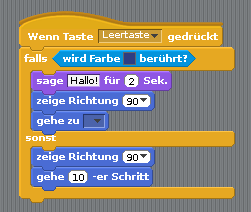
\includegraphics[width=0.6\textwidth]{images/aufgabe4_katze_bewegung_default.png}
\begin{itemize}
\item[3. ] Bei der Kachel \textit{Wenn Taste Leertaste gedrückt} klickst du auf den Text \textit{Leertaste} und w{\"a}hlst aus der Liste \textit{Pfeil nach oben}.
\item[4. ] Bei der Kachel \textit{wird Farbe berührt} auf die Farbe klicken und dann auf den grauen Rand unserer Rennbahn.
\item[5. ] Bei der Kachel \textit{sage Hallo! für 2 Sek.} auf den Text \textit{Hallo!} klicken und diesen zu \textit{Au!} ändern.
\item[6. ] Bei der Kachel \textit{zeige in Richtung 90} im \textit{falls}-Bereich auf die Zahl \textit{90} klicken und aus der Liste \textit{(-90) links} auswählen.
\item[7. ] Bei der Kachel \textit{gehe zu} auf den kleinen Pfeil klicken und unseren Sprite \textit{Start/Ziel} aus der Liste auswählen.
\item[7. ] Bei der Kachel \textit{zeige in Richtung 90} im \textit{sonst}-Bereich auf die Zahl \textit{90} klicken und aus der Liste \textit{(0) oben} auswählen.
\item[8. ] Bei der letzten Kachel \textit{gehe 10-er Schritt} soll die Zahl \textit{10} durch eine \textit{2} ersetzt werden.
\end{itemize}
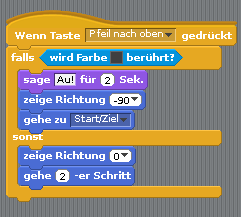
\includegraphics[width=0.6\textwidth]{images/aufgabe4_bewege_katze_nach_oben.png}

\begin{itemize}
\item[9. ] Das Ganze jeweils für die drei restlichen Richtungen \textit{rechts}, \textit{unten} und \textit{links} wiederholen und dabei nicht vergessen bei der Kachel \textit{zeige in Richtung 90} jeweils die gewünschte Richtung auswählen und die richtige Taste zu ändern.
\end{itemize}

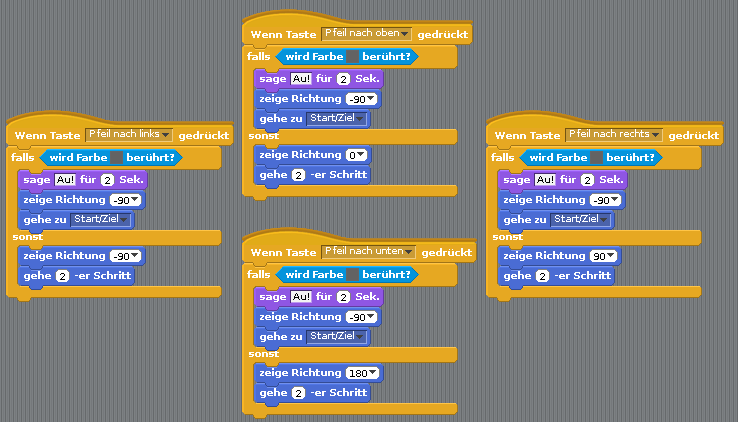
\includegraphics[width=0.6\textwidth]{images/aufgabe4_katze_alle_richtungen.png}
\begin{itemize}
\item[10. ] Um die Katze beim Start des Spiels zur Startlinie zu bringen, füge die Kacheln \textit{Wenn Fahne angeklickt} aus dem Steuerungs-Panel, aus dem Bewegungs-Panel \textit{zeige Richtung 90} und \textit{gehe zu} ein und setze diese zusammen.
\item[11. ] Bei der Kachel \textit{zeige in Richtung 90} im \textit{sonst}-Bereich auf die Zahl \textit{90} klicken und aus der Liste \textit{(-90) links} auswählen.
\item[12. ] Bei der Kachel \textit{gehe zu} auf den Pfeil klicken und aus dem Menü und \textit{Start/Ziel} auswählen.
\end{itemize}
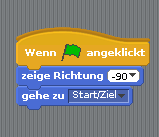
\includegraphics[width=0.6\textwidth]{images/aufgabe4_katze_an_start_stop.png}

\subsection{Zusatzaufgabe: Erweitere das Spiel damit zwei Spieler spielen können}
Du kannst einen weiteren Sprite hinzufügen und dir weitere vier Tasten auf der Tastatur aussuchen um diesen auch eine Steuerung zu geben. Hier die kurze Beschreibung wie man das machen könnte:
\begin{itemize}
\item[1. ] Die vier Tasten für die Steuerung überlegen z.B.
  \begin{itemize}
  \item w = oben
  \item d = rechts
  \item s = unten
  \item a = links
\end{itemize}
\item[2. ] Kopiere die Katze und passe die Skripte an, sodass die von dir ausgewählten Tasten zur Steuerung der Katze benutzt werden]
  \item[3. ] Ändere das Aussehen einer Katze um es leichter zu machen sie zu Unterscheiden (wir haben ihr ein paar Punkte gegeben).
\end{itemize}
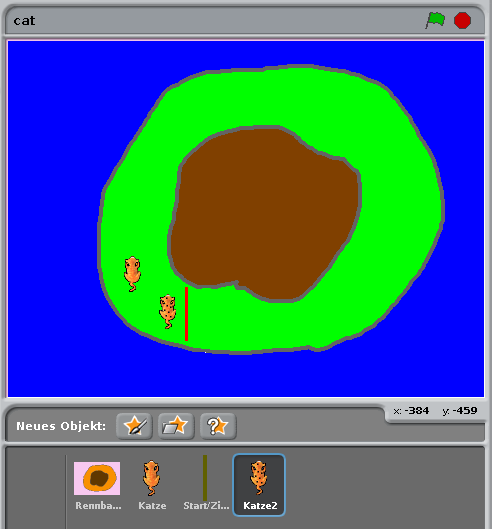
\includegraphics[width=0.6\textwidth]{images/aufgabe4_multiplayer.png}
